%%%%%%%%%%%%%%%%%%%%%%% file typeinst.tex %%%%%%%%%%%%%%%%%%%%%%%%%
%
% This is the LaTeX source for the instructions to authors using
% the LaTeX document class 'llncs.cls' for contributions to
% the Lecture Notes in Computer Sciences series.
% http://www.springer.com/lncs       Springer Heidelberg 2006/05/04
%
% It may be used as a template for your own input - copy it
% to a new file with a new name and use it as the basis
% for your article.
%
% NB: the document class 'llncs' has its own and detailed documentation, see
% ftp://ftp.springer.de/data/pubftp/pub/tex/latex/llncs/latex2e/llncsdoc.pdf
%
%%%%%%%%%%%%%%%%%%%%%%%%%%%%%%%%%%%%%%%%%%%%%%%%%%%%%%%%%%%%%%%%%%%


\documentclass[runningheads,a4paper]{llncs}

\usepackage{amssymb}
\setcounter{tocdepth}{3}
\usepackage{graphicx}
\usepackage{epstopdf}
\usepackage{mathtools}


\usepackage{url}
  
\newcommand{\keywords}[1]{\par\addvspace\baselineskip
\noindent\keywordname\enspace\ignorespaces#1}

\begin{document}

\mainmatter  % start of an individual contribution

% first the title is needed
\title{Constraint Satisfaction and Optimization Problem:\\Choosing Speakers for a Diversified Topic Conference}

% a short form should be given in case it is too long for the running head
\titlerunning{CSOP: Choosing Speakers for a Diversified Topic Conference}

% the name(s) of the author(s) follow(s) next
%
% NB: Chinese authors should write their first names(s) in front of
% their surnames. This ensures that the names appear correctly in
% the running heads and the author index.
%
\author{Carolina Centeio Jorge (up201403090)
\and Tiago Almeida (up20130565)}
%
\authorrunning{CSOP: Choosing Speakers for a Diversified Topic Conference}
% (feature abused for this document to repeat the title also on left hand pages)

% the affiliations are given next; don't give your e-mail address
% unless you accept that it will be published
\institute{FEUP-PLOG, 3MIEIC03,\\
Oradores Convidados 1\\
}

%
% NB: a more complex sample for affiliations and the mapping to the
% corresponding authors can be found in the file "llncs.dem"
% (search for the string "\mainmatter" where a contribution starts).
% "llncs.dem" accompanies the document class "llncs.cls".
%

\toctitle{Constraint Satisfaction and Optimization Problem}
\tocauthor{Choosing Speakers for a Diversified Topic Conference}
\maketitle


\begin{abstract}
%The abstract should summarize the contents of the paper and should
%contain at least 70 and at most 150 words. It should be written using the
\emph{This project aims to find the better set of speakers for a certain conference. The goal is to maximize the difference between topics (each speaker has a topic associated) considering some money, gender and country constraints. Since it is a Constraint Satisfaction and Optimization Problem, we used SICStus Prolog and the clp(FD) module.}
\keywords{CSOP, Prolog, clpfd, clp, constraint, logic programming, optimization}
\end{abstract}


\section{Introduction}

In the scope of the course PLOG, we were asked to implement a solution of a Constraint Satisfaction and Optimization Problem. Therefore, we chose “Invited Speakers” as subject to our project. This problem is similar to the “Production Management” problem, since we have to fulfill several constraints on the speakers’ diversity, but we need to maximize the difference amongst topics in the conference.\\
In this paper we will describe the problem in detail and its approach: decision variables (their domains and constraints), evaluation function and search strategy. In the end, we will present our solution, results and analyze them.


\section{Problem Description}

For a certain conference (that will take D days and T topics), there is the need to choose topics and speakers to talk about these topics. Each speaker has a name, a gender, a topic, a country, an travel expense and accommodation type associated.\\
There is a budget that cannot be exceeded. This budget will be used to pay speakers’ travel and accommodation expenses. The travel expense depends on the speaker and so does the accommodation, since one can choose to stay just for one night or for all conference (D nights).\\
Also, the speakers have to be equally distributed in gender and there cannot be two speakers coming from the same country. \\
All pairs of topics have a defined distance. The goal is to choose the speakers that maximize this distance amongst all topics in the conference.

\section{Approach}

To approach this problem, we create several lists with the speakers’ information. The lists Speakers, Topics, Countries, Gen, Desloc and Aloj have the information about names, topics, countries, gender, travel expense and type of accommodation of all possible speakers. We also create the list Invited, which contains the decision variables and the table of distances between all pairs of topics (Dist). The index determines the speaker in every list.

\subsection{Decision Variables}

In this project, the decision variables are the Boolean values for each speaker, that determines whether this is going to be chosen or not. Therefore, there are as many variables as possible speakers and their domain is Boolean (0 or 1). Ex: Invited = [I1,I2,I3], I1, I2 and I3 are the decision variables. I1 can be 1 or 0 meaning the speaker 1 is or is not going.

\subsection{Constraints}

\begin{itemize}
\item Only T speakers can be chosen (the sum of the decision variables has to match T).
\item There has to be the same number of male and female speakers (the scalar product of Gen and Invited has to be 0)
\item All invited speakers must come from different countries (If I[x] and I[y] are both 1, Countries[x] and Countries[y] must be different)
\item The travel and accommodation expenses (the sum of the scalar product of Desloc and Invited + (the sum of the scalar product of Desloc and Invited) * Night Price) must be covered by the budget ($<=$ budget).
\end{itemize}

\subsection{Evaluation Function}

Since we aim to find the maximum distance amongst topics, we calculate the sum of distances between the topics of all invited speakers (Invited is boolean, Distance is $>=$ 0).\\

$\sum_{i=1}^{T} Invited_i{ \sum_{j=i}^{T} Invited_j * Distance_{ij} }$ 

\subsection{Search Strategy}

We used maximize(Total) in labeling, in order to find the set of invited speakers that maximizes the function described above ( Total is the result of this function).

\section{Solution Presentation}

\begin{verbatim}
printResult([], _, _, _, _, _, _, _).

printResult([0|Is], [_|Ss], [_|Ts], [_|Cs], [_|Gs], [_|Ds], [_|As], DPrice) :-
        printResult(Is, Ss, Ts, Cs, Gs, Ds, As, DPrice).

printResult([1|Is], [S1|Ss], [T1|Ts], [C1|Cs], [G1|Gs], [D1|Ds], [A1|As], DPrice) :-
        nome(S1, Nome),
        pais(C1, Pais),
        genero(G1, Genero),
        topic(T1, Topic),
        Aloj is A1 * DPrice,
        write(Nome), write(' - '), write(Genero), write(' - '), write(Pais),
        write(' - '), write(Topic), write(' - '), write(D1), write(' - '), 
        write(Aloj), nl,
        printResult(Is, Ss, Ts, Cs, Gs, Ds, As, DPrice).
\end{verbatim}

\section{Results}
We ran the application eight times to study the relation between the execution time, resumptions, entailments, prunings, backtracks and the number of lectures. Throughout the eight executions, the number of possible speakers was 20. 

\begin{figure}[!h]
\centering
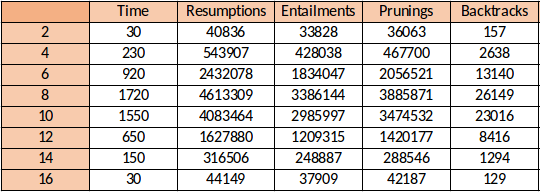
\includegraphics[width=10.9cm,height=3.8cm]{Table1}
\caption{Time, Resumptions, Entailments, Prunings and Backtracks depending on the number of lectures.}
\label{fig:Table1}
\end{figure}

\begin{figure}[!h]
\centering
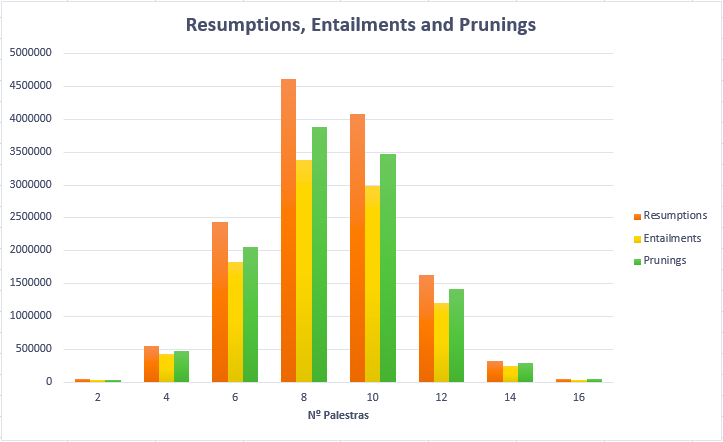
\includegraphics[width=11.5cm,height=7cm]{Graph1}
\caption{Resumptions, Entailments and Pruning Graph.}
\label{fig:Graph1}
\end{figure}

\begin{figure}[!h]
\centering
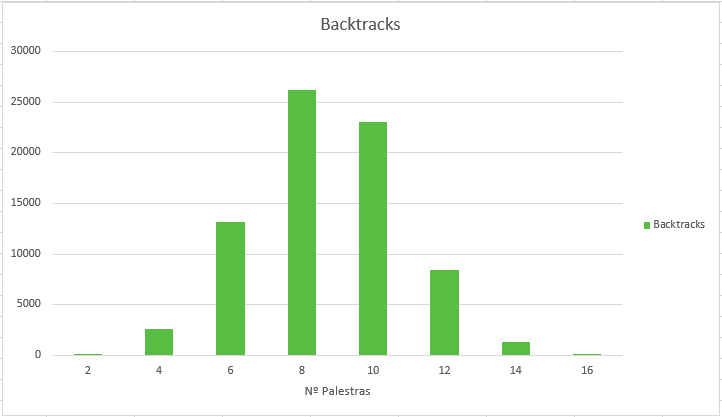
\includegraphics[width=11.5cm,height=7cm]{Backtracks}
\caption{Backtracks Graph.}
\label{fig:Graph1}
\end{figure}

\begin{figure}[!h]
\centering
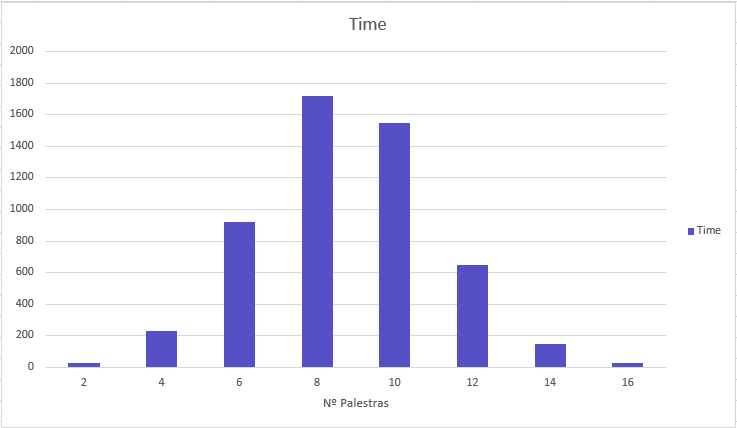
\includegraphics[width=11.5cm,height=7cm]{Time}
\caption{Time Graph.}
\label{fig:Graph1}
\end{figure}

\clearpage
As we can see, all graphs have a similar distribution. The program finishes execution in less than a second when the number of lectures are  2, 4, 6, 12, 14 or 16. However, when the number of lectures are 8 or 10, the programs takes more than one second to execute. This behavior was already predicted and it can be easily explained with the Pascal's Triangle. The number of possible solutions increases the closest the number of lectures is to the average, therefore, to maximize the solution, it is necessary to process more possibilities, which takes more time.

\begin{figure}[!h]
\centering

\includegraphics[width=4cm,height=3cm]{Pascal}
\caption{Pascal Triangle example from 1 to 5 number of lectures.}
\label{fig:Graph1}
\end{figure}

\begin{figure}[!h]
\centering
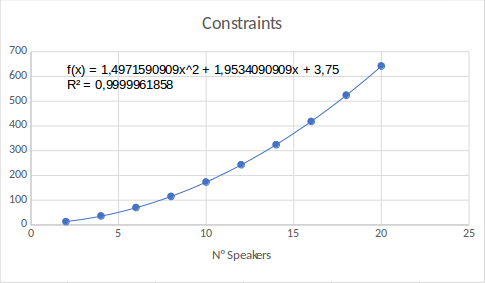
\includegraphics[width=9cm,height=6cm]{Constraints}
\caption{Number of constraints depending on the number of available speakers.}
\label{fig:Graph1}
\end{figure}

As seen above, the number of constraints follows a quadratic distribution depending on the number of available speakers. Although most restrictions follow a linear evolution curve, the country restriction follows a quadratic one. For every possible pair of possible speakers, we need to force them to have different countries, therefore adding one speaker to the database implies adding N more country restrictions, N being the number of available speakers.
\end{document}
